\documentclass{beamer}
\usepackage{siunitx}
\usepackage{tfrupee}
\renewcommand{\vec}[1]{\mathbf{#1}}
\mode<presentation>
\usepackage{amsmath}
\usepackage{amssymb}
%\usepackage{advdate}
\usepackage{adjustbox}
%\usepackage{subcaption}
\usepackage{multicol}
\usepackage{mathtools}
\usepackage{listings}
\usepackage{url}
\usetheme{Boadilla}
\usecolortheme{lily}
\setbeamertemplate{footline}
{
  \leavevmode%
  \hbox{%
  \begin{beamercolorbox}[wd=\paperwidth,ht=2.25ex,dp=1ex,right]{author in head/foot}%
    \insertframenumber{} / \inserttotalframenumber\hspace*{2ex} 
  \end{beamercolorbox}}%
  \vskip0pt%
}
\setbeamertemplate{navigation symbols}{}
\providecommand{\nCr}[2]{\,^{#1}C_{#2}} % nCr
\providecommand{\nPr}[2]{\,^{#1}P_{#2}} % nPr
\providecommand{\mbf}{\mathbf}
\providecommand{\pr}[1]{\ensuremath{\Pr\left(#1\right)}}
\providecommand{\qfunc}[1]{\ensuremath{Q\left(#1\right)}}
\providecommand{\sbrak}[1]{\ensuremath{{}\left[#1\right]}}
\providecommand{\lsbrak}[1]{\ensuremath{{}\left[#1\right.}}
\providecommand{\rsbrak}[1]{\ensuremath{{}\left.#1\right]}}
\providecommand{\brak}[1]{\ensuremath{\left(#1\right)}}
\providecommand{\lbrak}[1]{\ensuremath{\left(#1\right.}}
\providecommand{\rbrak}[1]{\ensuremath{\left.#1\right)}}
\providecommand{\cbrak}[1]{\ensuremath{\left\{#1\right\}}}
\providecommand{\lcbrak}[1]{\ensuremath{\left\{#1\right.}}
\providecommand{\rcbrak}[1]{\ensuremath{\left.#1\right\}}}
\theoremstyle{remark}
\newtheorem{rem}{Remark}
\newcommand{\sgn}{\mathop{\mathrm{sgn}}}
\usepackage{enumitem}
\providecommand{\res}[1]{\Res\displaylimits_{#1}} 
\providecommand{\norm}[1]{\left\lVert#1\right\rVert}
\providecommand{\mtx}[1]{\mathbf{#1}}
\providecommand{\abs}[1]{\left\vert#1\right\vert}
\providecommand{\fourier}{\overset{\mathcal{F}}{ \rightleftharpoons}}
%\providecommand{\hilbert}{\overset{\mathcal{H}}{ \rightleftharpoons}}
\providecommand{\system}{\overset{\mathcal{H}}{ \longleftrightarrow}}
	%\newcommand{\solution}[2]{\textbf{Solution:}{#1}}
%\newcommand{\solution}{\noindent \textbf{Solution: }}align
\providecommand{\dec}[2]{\ensuremath{\overset{#1}{\underset{#2}{\gtrless}}}}
\newcommand{\myvec}[1]{\ensuremath{\begin{pmatrix}#1\end{pmatrix}}}

\title{Matrices in Geometry - 5.13.63}
\author{EE25BTECH11037  Divyansh}
\date{Sept, 2025}

\begin{document}

\maketitle


\section{Problem}
\begin{frame}
\frametitle{Problem Statement}
Let $\vec{M}=\myvec{\sin^4\brak{\theta} & -1-\sin^2\brak{\theta} \\ 1+\cos^2\brak{\theta} & \cos ^4\brak{\theta}} = \alpha \vec{I} + \beta\vec{M}^{-1} $\\
Where $\alpha = \alpha\brak{\theta}$ and $\beta = \beta \brak{\theta}$ are real numbers, and $\vec{I}$ is the $2 \times 2$ identity matrix.
If $\alpha^*$ is the minimum of the set 
    $\brak{\alpha\brak{\theta}: \theta \in [0, 2\pi)} $ and $\beta^*$ is the minimum of the set
$\brak{\beta\brak{\theta} : \theta \in [0, 2\pi)}$. Then the value of $\alpha^* + \beta^*$ is
\begin{enumerate}[label=(\alph*)]
    \item $-\frac{31}{16}$
    \item $-\frac{17}{16}$
    \item $-\frac{37}{16}$
    \item $-\frac{29}{16}$
\end{enumerate}
\end{frame}

\section{Solution}
\begin{frame}{Solution}
Using the Cayley-Hamilton Theorem, 
\begin{align}
    \vec{M}^2 - tr\brak{\vec{M}}\vec{M} + det\brak{\vec{M}}\vec{I}=0\\
    \implies \vec{M} -tr\brak{\vec{M}}\vec{I} + det\brak{\vec{M}}\vec{M}^{-1} =0
\end{align}
The given expression is
\begin{align}
    \vec{M} -\alpha\vec{I} - \beta\vec{M}^{-1} =0
\end{align}
\end{frame}

\begin{frame}{Solution}
On comparing, we get
\begin{align}
    \alpha = tr\brak{\vec{M}} \ , \ \beta = - det\brak{\vec{M}}\\
    \alpha\brak{\theta}=\sin^4\brak{\theta}+\cos^4\brak{\theta} = 1-2\sin^2\brak{\theta}\cos^2\brak{\theta}\\
    \implies \alpha = 1 -\sin^2\brak{2\theta}/2 \\
    \alpha^*  = min\brak{\alpha\brak{\theta}}= 1- 1/2 = \frac{1}{2} ,\\ \brak{\because \text{for minimizing $\alpha$,  $\sin^2\brak{2\theta}$ should be maximum}}\nonumber\\
    \beta\brak{\theta} = - det\brak{\vec{M}} = - \brak{\sin^4\brak{\theta}\cos^4\brak{\theta} + \sin^2\brak{\theta}\cos^2\brak{\theta} +2}\\
    \implies \beta = - \brak{ \brak{\sin\brak{2\theta}/2}^4 + \brak{\sin\brak{2\theta}/2}^2 + 2} \\
    \beta^* = - \brak{ \brak{1/2}^4 + \brak{1/2}^2 + 2}=--\frac{37}{16}\\
    \brak{\because \text{for minimizing $\beta$,  $\sin^2\brak{2\theta}$ should be maximum}}\nonumber
\end{align}
\end{frame}
\begin{frame}{Solution}
    Now, 
\begin{align}
    \alpha^*+\beta^* = \frac{1}{2} - \frac{37}{16} = -\frac{29}{16}
\end{align}
Thus,  the correct option is option $\brak{d}$\\
We get $\alpha^*, \beta^*$ at $\theta = \frac{\pi}{4}$, substituting this in $\vec{M}$, we get
\begin{align}
    \vec{M}=\myvec{\brak{\frac{1}{\sqrt{2}}}^ 4 & -1-\brak{\frac{1}{\sqrt{2}}}^2 \\  1+\brak{\frac{1}{\sqrt{2}}}^2 & \brak{\frac{1}{\sqrt{2}}}^ 4} = \myvec{\frac{1}{4} & \frac{-3}{2} \\ \frac{3}{2} &\frac{1}{4}}
\end{align}
Let us draw graphs to find $\alpha^*, \beta^*$:
\end{frame}
\begin{frame}{Graph for Alpha}
    \begin{figure}
    \centering
    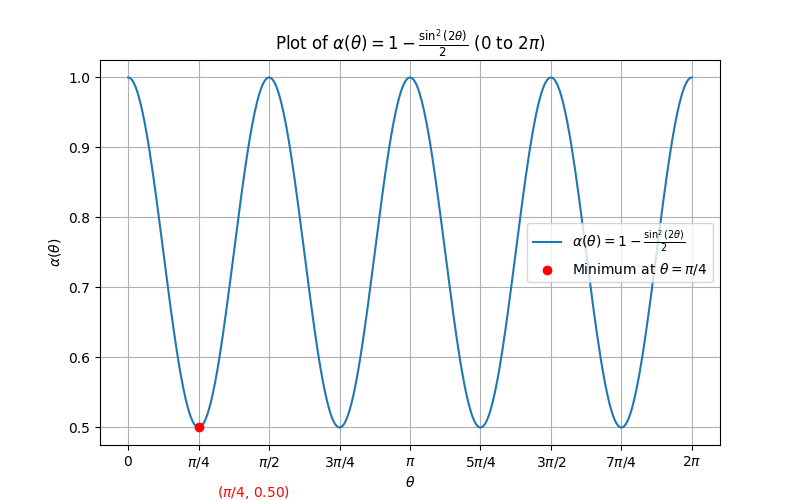
\includegraphics[width=0.5\columnwidth]{figs/alpha.png}
    \caption{Graph for $\alpha\brak{\theta}$}
    \label{fig:placeholder}
\end{figure}
\end{frame}
\begin{frame}{Graph for Beta}
    \begin{figure}
    \centering
    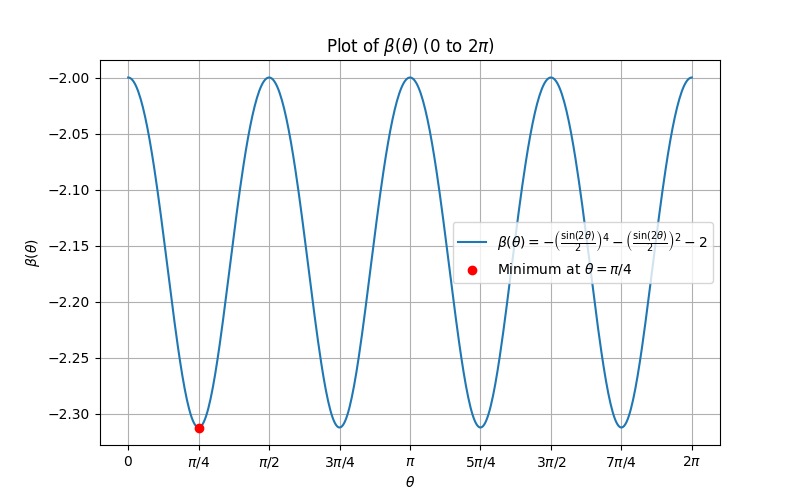
\includegraphics[width=0.5\columnwidth]{figs/beta.png}
    \caption{Graph for $\beta\brak{\theta}$}
    \label{fig:placeholder}
\end{figure}
\end{frame}

\end{document}